\documentclass[%
	paper=A4,					% paper size --> A4 is default in Germany
	twoside=false,				% onesite or twoside printing
	openright,					% doublepage cleaning ends up right side
	parskip=full,				% spacing value / method for paragraphs
	chapterprefix=true,			% prefix for chapter marks
	12pt,						% font size
	headings=normal,			% size of headings
	bibliography=totoc,			% include bib in toc
	listof=totoc,				% include listof entries in toc
	titlepage=off,				% own page for each title page
	captions=tableabove,		% display table captions above the float env
	draft=false,				% value for draft version
]{scrreprt}%

% **************************************************
% Debug LaTeX Information
% **************************************************
%\listfiles

% **************************************************
% Information and Commands for Reuse
% **************************************************
\newcommand{\thesisTitle}{The Clean Thesis Style}
\newcommand{\thesisName}{Ricardo Langner}
\newcommand{\thesisSubject}{Documentation}
\newcommand{\thesisDate}{April 7, 2014}
\newcommand{\thesisVersion}{0.2.3}

\newcommand{\thesisFirstSupervisor}{Jane Doe}

\newcommand{\thesisUniversity}{\protect{Clean Thesis Style University}}
\newcommand{\thesisUniversityDepartment}{Department of Clean Thesis Style}
\newcommand{\thesisUniversityInstitute}{Institut for Clean Thesis Dev}

% **************************************************
% Load and Configure Packages
% **************************************************
\usepackage{subcaption}
\usepackage{fixmath}
\usepackage{float}
\usepackage[utf8]{inputenc}		% defines file's character encoding
\usepackage[english]{babel} % babel system, adjust the language of the content
\usepackage[					% clean thesis style
	figuresep=colon,%
	sansserif=false,%
	hangfigurecaption=false,%
	hangsection=true,%
	hangsubsection=true,%
	colorize=full,%
	colortheme=bluemagenta,%
]{cleanthesis}

\hypersetup{					% setup the hyperref-package options
	pdftitle={\thesisTitle},	% 	- title (PDF meta)
	pdfsubject={\thesisSubject},% 	- subject (PDF meta)
	pdfauthor={\thesisName},	% 	- author (PDF meta)
	plainpages=false,			% 	- 
	colorlinks=false,			% 	- colorize links?
	pdfborder={0 0 0},			% 	-
	breaklinks=true,			% 	- allow line break inside links
	bookmarksnumbered=true,		%
	bookmarksopen=true			%
}
\usepackage{graphicx}
\graphicspath{ {gfx/} }
%------------double page settings
\iffalse

\usepackage{geometry}
 \geometry{
 left=25mm,
 right=25mm,
 top=20mm,
 bottom=20mm,
}
\addtolength{\oddsidemargin}{5mm}
\addtolength{\evensidemargin}{-5mm}

\fi
% **************************************************
% Document CONTENT
% **************************************************
\begin{document}

% --------------------------
% rename document parts
% --------------------------
%\renewcaptionname{ngerman}{\figurename}{Abb.}
%\renewcaptionname{ngerman}{\tablename}{Tab.}
\renewcaptionname{english}{\figurename}{Fig.}
\renewcaptionname{english}{\tablename}{Tab.}

% --------------------------
% Front matter
% --------------------------
\pagenumbering{roman}			% roman page numbing (invisible for empty page style)
\pagestyle{empty}				% no header or footers
%----------------------------------Main Titlte page
% Last modified on 6th May 2006
\begin{titlepage}
\begin{center}
\vspace{0.1in}
\Large{ MM 640: Modelling of Microstructural evalution \\ Midsem Project}\\
\vspace{0.6in}

{\Huge {\bf 
Phase field study of \\ grain boundary\\ 
\vspace{0.1in}
effects on spinodal decomposition }} \\
\vspace{0.5in}

%{\bf Thesis} \\ [1ex]
%{\bf Synopsis} \\ [1ex]

by\\
\vspace{0.2in}
{\bf Yash Agarwal\\(12D110054)} \\ 
\vspace{0.5in}
Guide: \\ 
%Under the guidence of \\ 
%\vspace{0.1in}
Prof. M.P. Gururajan\\
\vspace{0.3in}
%\newfont{\iitblogofont}{iitblogo}{\iitblogofont a \\}

\includegraphics[scale=0.12]{iitb_logo}\\
\vspace{0.1in}
{\normalsize
Department of Metallurgical Engineering and Materials Science\\ 

\vspace{2mm}
INDIAN INSTITUTE OF TECHNOLOGY BOMBAY\\
\vspace{3mm}
Aug-Oct,2015 \\
}
\end{center}
\thispagestyle{empty}
\end{titlepage}

		% INCLUDE: all titlepages
\cleardoublepage

\pagestyle{plain}				% display just page numbers
%% !TEX root = Clean-Thesis.tex
%
\pdfbookmark[0]{Abstract}{Abstract}
\chapter*{Abstract}
\label{sec:abstract}
\vspace*{10mm}


\textit{\large
Unique nature of disordered structure in Metallic Glasses provides the combination of exceptional physical properties like at one end they are among the hardest materials ever made while on the other end pretty easier to work and form despite their hardness. Due to the lack of long range periodicity and related grain boundaries with defects, Metallic Glasses are reaching the limits of the theoretical strength. Their net shape processability by Cu-mold casting, suction casting and super plastic forming in Newtonian viscous flow regime (supercooled region) have led these materials to replicate in small features and in thin sections with high aspect ratios. Also, Metallic Glasses do not require post-cast processing or heat treatment, as all properties are already achieved in as-cast state. Also they could be fabricated and processed at lower temperatures comparative to their crystalline counterparts. Almost zero shrinkage during fabrication for these alloys makes them perfect for precision casting. These ideal properties have made possible their use in a number of fields ranging from very sophisticated tools like micro-geared motors to major commercial applications in the present world. The major applications of these precious metals are in sports items, hard casings, aircrafts, surgical instruments, industrial coatings and energy savings as amorphous core transformers and in various kind of sensors i.e. pressure sensor in auto mobile industry for injection control, oil pressure control, air conditioning, clogging monitor, brake control, and magnetic and magneto-optical sensors i.e. current sensation and optical communication.
}
		% INCLUDE: the abstracts
\cleardoublepage
%
%% !TEX root = ../thesis-example.tex
%
\pdfbookmark[0]{Acknowledgement}{Acknowledgement}
\chapter*{Acknowledgement}
\label{sec:acknowledgement}
\vspace{10mm}
{\large
I thank Prof Ajit Kulkarni who provided insight and expertise that greatly assisted the success of the project.  I thank him for sharing his pearls of wisdom with us during the course of this project. I would like to show my gratitude to  my colleagues for their assistance and comments that greatly improved  the  manuscript.  . . }



 % INCLUDE: acknowledgement
\cleardoublepage
%
\setcounter{tocdepth}{2}		% define depth of toc
\tableofcontents				% display table of contents
\cleardoublepage

% --------------------------
% Body matter
% --------------------------
\pagenumbering{arabic}			% arabic page numbering
\setcounter{page}{1}			% set page counter
\pagestyle{maincontentstyle} 	% fancy header and footer

\chapter{Introduction}

This is a part reproduction of the paper \textbf{"Phase field study of grain boundary effects on spinodal decomposition, Acta Materialia, 2003"}  by H. Ramanarayan, T.A. Abinandanan of Department of Metallurgy, IISc, Bangalore, India.
The authors of the above mentioned paper developed a phase field model of a polycrystalline binary alloy by combining the following:
\begin{enumerate}
\item The \textbf{Cahn–Hilliard} model(for conserved variables) for a compositionally inhomogeneous alloy.
\item A model of polycrystals (Fan D, Chen L-Q. Acta Mater. 1997;45:3297) which is governed by the Cahn–Allen equation for non-conserved variables 
 \end{enumerate} 

Further, this Model was used to study grain boundary (GB) effects on spinodal decomposition (SD) in two-dimensional (2D) systems. \\
This report goes throught the explanantion of the Model developed and the implementation of the simulations(codes attached) together with an comparison of results obtained in the paper with those obtained in the reproduction.


\chapter{Model}

\section{Cahn Hilliard Model}
Cahn–Hilliard Model for a compositionally inhomogeneous alloy is used. It is developed using the composition field \textbf{c(r)} in an alloy. The local composition \textbf{c} used in this model is defined as follows: 

\begin{equation}
\mathbold{
\frac{c^{'}-c^{'}_{\alpha}}{c^{'}_{\beta}-c^{'}_{\alpha}}
}
\end{equation}

where, $\mathbold{c^{'}}$ is the local composition,\\
$\mathbold{c^{'}_{\alpha}}$ is the equilibrium composition of the A rich $\mathbold{\alpha}$ phase,\\
$\mathbold{c^{'}_{\beta}}$ is the equilibrium composition of the B rich $\mathbold{\beta}$ phase,\\
all the above values are expressed in mole fraction of species B. Thus, for $\mathbold{\alpha}$ phase $\mathbold{c = 0}$ and for $\mathbold{\beta}$ phase $\mathbold{c = 1}$


\section{Cahn Allen Model}
Cahn–Allen theory for non-conserved variables (the model of Fan and Chen (1997) belongs to this category) is used. It is developed using a set of \textbf{n} 'orientational' (and non-conserved) order parameter fields $\mathbold{\eta_{i}(r) (i =1,2,...,n) }$to represent \textbf{n} different grain orientations in the microstructure; $\mathbold{\eta_{i}}$ are continuum analogues of Potts variables in the \textbf{n}-state Potts model

Each $\mathbold{\eta_{i}}$ is taken to be 1 within the $i^{th}$ grain and drops
to 0 outside it, through a GB region where it varies smoothly.

\begin{figure}[H]
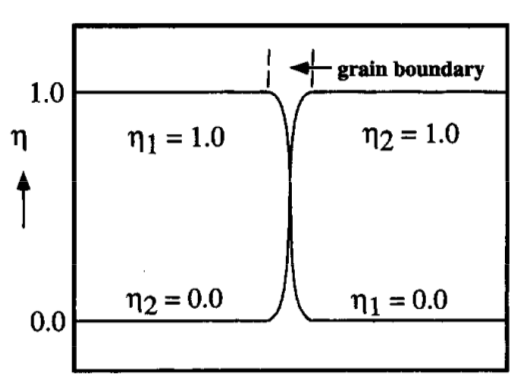
\includegraphics[scale=0.7]{gbProfile}
\caption{The schematic profiles of two orientation variables across a flat grain boundary}
\end{figure}

\section{Conclusion}
An instantaneous configuration in our model is described in terms of the \textbf{n+1} position-dependent field variables $\mathbold{(c;\eta_1, \eta_2, …….., \eta_n)}$.


\chapter{Mathematical Formulation of the Model}

\section{Energetics}
The Total Free energy, \textbf{F}, of a system with inhomogeneities in both \textbf{c} and $\mathbold{\eta_{i}}$ is written as a volume integral:

\begin{equation}
F=N_V\int\left[f(c,\eta_i)+ \kappa(\nabla c)^2 +\sum_i^n \kappa(\nabla \eta_i)^2    \right] 
\end{equation}

where, 
$\mathbold{N_V}$ is the (constant) number of atoms per unit volume,
$\mathbold{f(c,\eta_{i})}$ is the bulk free energy density and, 
$\mathbold{\kappa_{c}}$ and $\mathbold{\kappa_{i}}$ are the (constant) gradient energy coefficients associated with inhomogeneities in \textbf{c} and in $\mathbold{\eta_{i}}$ , respectively. 
It is assumed that $\mathbold{\kappa_{i}=\kappa_{\eta}}$ for all i.

Thus, the bulk free energy density $\mathbold{f(c,\eta_{i})}$ is chosen such that it exhibits a minimum for these \textbf{2n} possibilities. In other words, \textbf{f} has \textbf{2n} degenerate minima (whose value is chosen to be 0). 
These minima are located at \textbf{n} grains of  $\mathbold{\alpha}$ with a composition of $\mathbold{c = 0:(0;1,0,...,0), (0;0,1,...,0),...,(0;0,0,...,1),}$ and \textbf{n} grains of $\mathbold{\beta}$ with a composition of \\
$\mathbold{c = 1:(1;1,0,...,0), (1;0,1,...,0),...,(1;0,0,...,1).}$

%equation

\begin{equation}
f(c,\eta_i)=f(c_o)+m(c)\left\{  0.25+\sum_i^n \left[- \frac{\eta_i^2}{2}+ \frac{\eta_i^4}{4}\right] + \epsilon\sum_i^n\sum_{j>i}^n \eta_i^2\eta_j^2 \right\}
\end{equation}


$\mathbold{f_o(c)}$ is the free energy per atom in a bulk single crystal of composition \textbf{c} given by: The constant $\mathbold{A_c}$ determines the height of the free energy barrier between the equilibrium phases within a single grain, $\mathbold{m(c)}$ is a composition dependent factor which couples \textbf{c} and $\mathbold{\eta_{i}}$ and $\mathbold{\epsilon}$ is a constant. 

%%equation

\begin{equation}
f(c_o)=A_c c^2(1-c)^2
\end{equation}

\begin{equation}
f(c,\eta_i)=f(c_o)+m(c)\left\{  0.25+\sum_i^n \left[- \frac{\eta_i^2}{2}+ \frac{\eta_i^4}{4}\right] + \epsilon\sum_i^n\sum_{j>i}^n \eta_i^2\eta_j^2 \right\}
\end{equation}


Note that the terms within the curly braces are even functions of $\mathbold{\eta_{i}}$ ; therefore, $\mathbold{f(c,\eta_{i})}$ has additional degenerate minima at \textbf{2n} more locations with negative values of $\mathbold{f(c,\eta_{i})}$ such as $\mathbold{{c ;\eta_{i}} = (0;-1,0,...,0),...}$. In this case, these extra degenerate equilibrium states are excluded by working only with $\mathbold{\eta_{i}\geq 0}$.

\section{Kinetics}
The evolution of the composition field \textbf{c} is governed by the Cahn–Hilliard equation for conserved variables:

%equation

\begin{equation}
\frac{\partial c}{\partial t}=M\nabla^2\left[\frac{\partial \frac{F}{N_V}}{\partial c}\right]
\end{equation}

where $\mathbold{\frac{\partial \frac{F}{N_V}}{\partial c}=\mu}$ is the chemical potential whose gradient drives diffusion, and \textbf{M} is the atomic mobility.

The evolution of order parameter fields $\mathbold{\eta_{i}}$ is governed by the Cahn–Allen equation for non-conserved variables:

%equations
\begin{equation}
\frac{\partial \eta_i}{\partial t}=-L_i\left[\frac{\partial \frac{F}{N_V}}{\partial \eta_i}\right]
\end{equation}

where $\mathbold{\frac{\partial \frac{F}{N_V}}{\partial \eta_i}}$ is the total free energy (per atom) with respect to $\mathbold{\eta_{i}}$ , and $\mathbold{L_{i}}$ are the relaxation coefficients for $\mathbold{\eta_{i}}$ . Here, \textbf{M} and $\mathbold{L_i= L (i = 1,2,...,n)}$ are assumed to be constants.

\section{Numerical Implementation}

\begin{equation}
\frac{\partial c}{\partial t}=M\nabla^2\left[g(c)-2\kappa_c\nabla^4 c\right]
\end{equation}

where $\mathbold{g(c)=\frac{\partial f}{\partial c}}$
The numerical method used in our simulations is based on the semi-implicit Fourier spectral method

\begin{equation}
\tilde{c}(k,t+\triangle t)=\frac{\tilde{c}(k,t)-\triangle t M k^2 \tilde{g}(k,t)}{1+2\triangle t M \kappa_c k^4}
\end{equation}

Similarly for the Cahn–Allen equation

\begin{equation}
\tilde{\eta_i}(k,t+\triangle t)=\frac{\tilde{\eta_i}(k,t)-\triangle t L_i \tilde{h_i}(k,t)}{1+2\triangle t L_i \kappa_\eta k^2}
\end{equation}

where $\mathbold{h_i=\frac{\partial f}{\partial \eta_i}}$


\chapter{Settings for Simulation}

\section{The values of the parameters}

\begin{figure}[H]
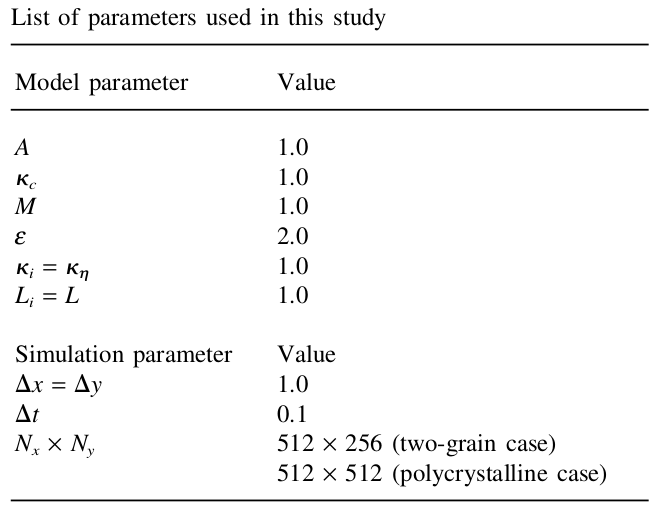
\includegraphics[width=\linewidth]{paraTable}
\caption{The value of all parameters chosen for this stuudy}
\end{figure}

\section{Variation of $\mathbold{m(c)}$ and $\mathbold{\delta_c}$(disturbance)}
The Initial Profile is set by $\mathbold{c_o=0.5 +- \delta_c}$
$\mathbold{\delta_c}$ is varied from 0.01 to 0.04

4 diffirent cases have been defined for which the parameters are chosen as follows

\begin{figure}[H]
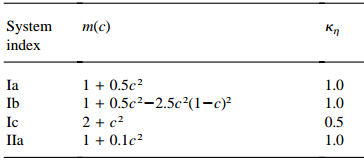
\includegraphics[scale=0.9]{some}
\caption{The system definitions for the study}
\end{figure}



\chapter{Pseudo Code}
This is the general code for which minor changes are made to get the complete results.
\begin{verbatim}
Take input from file input.dat
n_x, delta_x, n_y, delta_y, T, delta_t, T_write
(after how many steps do we print the output in a file)
Declare composition,n1,n2,g,h1 & h2 matrix and Allocate memory
Declare the Fourier Transform's respectively

Calculate half_nx, half_ny, delta_kx & delta_ky

Make the Initial Profile
Traverse the matrix
      Generate Random Number R=[-1,1]
      composition=0.5 +- R*0.04
			IF i<half_nx
			   n1=1 & n2=0
			ELSE
        	   n1=0 & n2=1
Start time loop
Traverse Matrix
Calculate g,h1,h2
Take composition,n1,n2,g,h1 & h2 to Fourier space
Evolve composition    
Traverse Matrix
        	Calculate kx,ky
        	Calculate new composition,n1 & n2 -- 
    	Take composition,n1 & n2 back to real space
    	Traverse Matrix
        Normalise the values and Set imaginary part to zero 
        for composition,n1 & n2
    After every T_write time steps write composition profile to file
end time loop
Free all memory
\end{verbatim}
\chapter{Results}
The results have been summarized in the following sections and the code files are also provided specific to each section.

\section{GB effects in a two-grain system}
In this Figure we show the evolution of microstructure in a two-grain system (with periodic boundary conditions along both x and y axes) in system \textbf{Ia}(a defined earlier) for \textbf{t=10, 50 and 200}, for an alloy of composition $\mathbold{c_o = 0.5}$ and with initial fluctuations of $\mathbold{\delta_c = 0.04}$. For this system, $\mathbold{\gamma_\alpha}$, the $\mathbold{\alpha}$-GB energy is about 18\% lower than $\mathbold{\gamma_\beta}$. This difference provides the driving force, during early stages, for the GB to acquire species A.

This process of GB enrichment with species A also leads to the formation of a B-enriched layer (white band) followed by a faint A-rich band (dark grey) on either side of the boundary in the figure. During this time, the grain interior undergoes normal SD; the extent of this decomposition, however, is much smaller than that at the boundaries. At t = 50, the microstructure shows three bands at and near the GB in each grain (starting with the $\mathbold{\alpha}$ band at the GB, followed by a $\mathbold{\beta}$ band and a second $\mathbold{\alpha}$ band), coexisting with a grain interior exhibiting normal SD.
\begin{figure}[H]
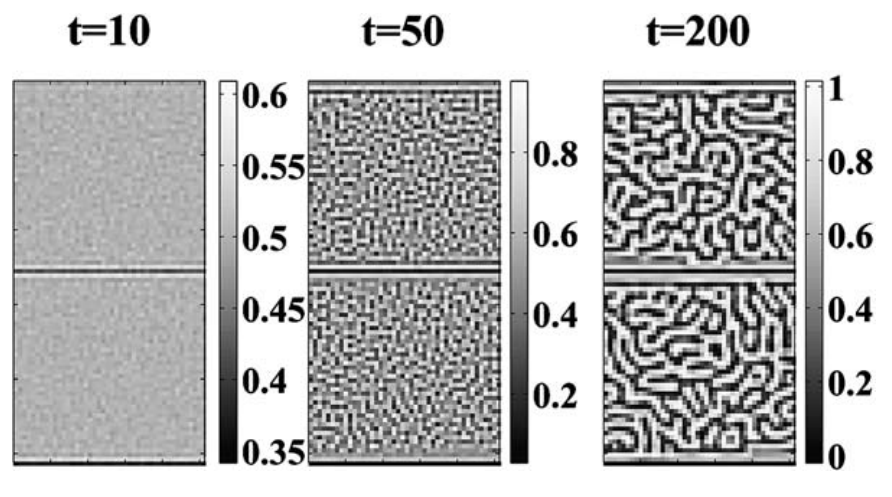
\includegraphics[width=\linewidth]{Fig2A}
\caption{Actual Figure}
\end{figure}

\begin{figure}[H]
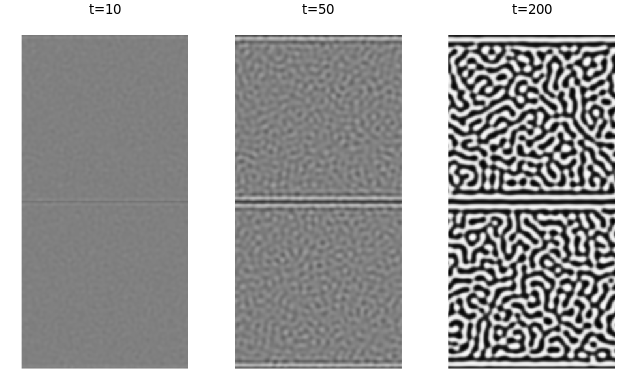
\includegraphics[width=\linewidth]{Fig2}
\caption{Reproduced Figure}
\end{figure}

\section{Effect of ($\mathbold{\gamma_\beta-\gamma_\alpha}$) and initial fluctuation}
The microstructural evolution depicted in the above figure may be described in terms of a competition
between two different phenomena: 
\begin{enumerate}
\item GB assisted phase separation which initiates a composition wave which travels into the grains and is faster than the other
\item normal SD in the grain interior which leads to the formation of a bicontinuous microstructure of A-rich and B-rich regions
\end{enumerate}

From the results(as shown in figure) we may infer that the number of bands near the GB would be 
\begin{enumerate}
\item higher if the normal SD in grain interiors can be delayed (e.g., by using smaller fluctuations (noise) in the initial configuration), and  
\item lower if the driving force (gamma|beta-gamma|alpha) for the GB enrichment with species A is made smaller. \end{enumerate}

We test these hypothesis in this section\\
We compare the following 3 systems at t=100
\begin{enumerate}

\item System Ia @ $\mathbold{\delta_c = 0.04}$; this represents a high driving force for the GB enrichment, and high initial noise. It shows three bands in each grain.
\item System Ia @ $\mathbold{\delta_c = 0.01}$; similar to the later case but with a lower initial noise which delays normal SD and allows for GB assisted phase separation. It shows 5 bands.
\item System IIa @ $\mathbold{\delta_c = 0.01}$; Same lower initial noise together with further reduced driving force which reduces the GB assisted phase separation compared to the previous phase and so we only see 4 bands.

\end{enumerate}

\begin{figure}[H]
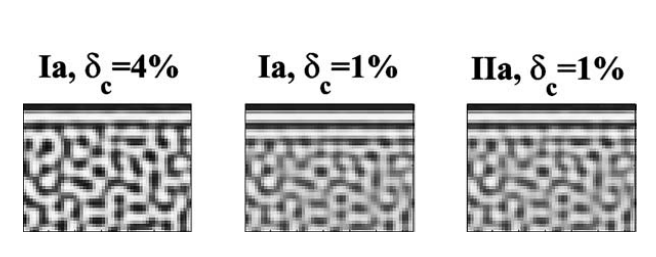
\includegraphics[width=\linewidth]{Fig3A}
\caption{Actual Figure}
\end{figure}

\begin{figure}[H]
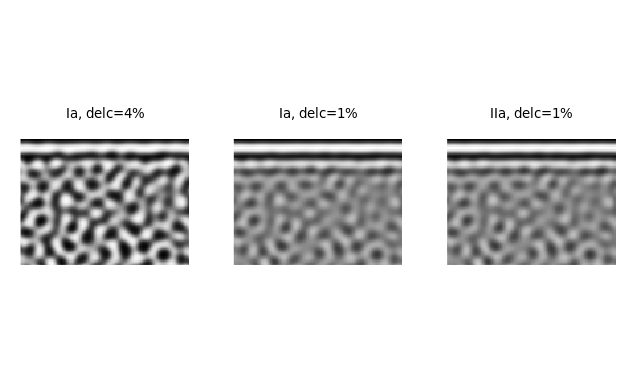
\includegraphics[width=\linewidth]{Fig3}
\caption{Reproduced Figure}
\end{figure}

\subsection{Analysis of deviation of composition from average composition with distance from the GB}
The difference $\mathbold{c_p-c_o}$ as a function of distance from the GB, where $\mathbold{c_p}$ is the average composition within a layer parallel to the GB and $\mathbold{c_o}$ is the alloy composition. The figure below shows that the composition wave is initiated at the GB, and propagates into the grain interiors; further, for a given time, this composition wave also decays with distance from the GB.

\begin{figure}[H]
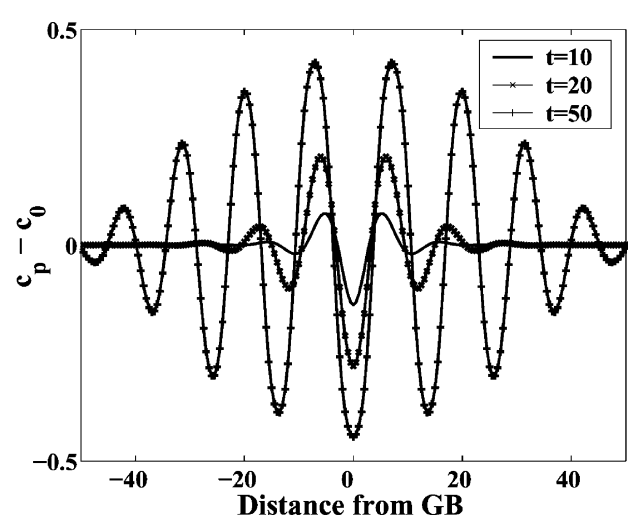
\includegraphics[width=\linewidth]{Fig4A}
\caption{Actual Figure}
\end{figure}

\begin{figure}[H]
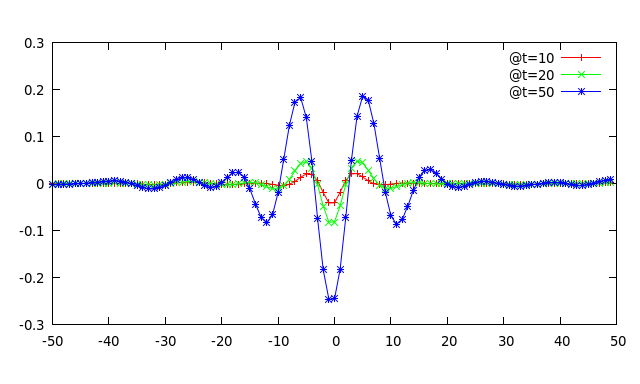
\includegraphics[width=\linewidth]{Fig4}
\caption{Reproduced Figure}
\end{figure}

\subsection{$R_1$(t) vs t}

$\mathbold{R_1(t)}$, the first zero of the $\mathbold{c_p-c_o}$ profile, is plotted as a function of time for systems Ia, lb and Ic. It is clear that $\mathbold{R_1}$ increases with time, before stabilizing towards late stages. More importantly, the $\mathbold{R_1(t)}$ behaviour is essentially the same in these three systems, indicating that differences in GB widths (in system Ic) or in incoherent boundary energy (in system Ib) do not play a significant role in determining the formation of GB-bands.

\begin{figure}[H]
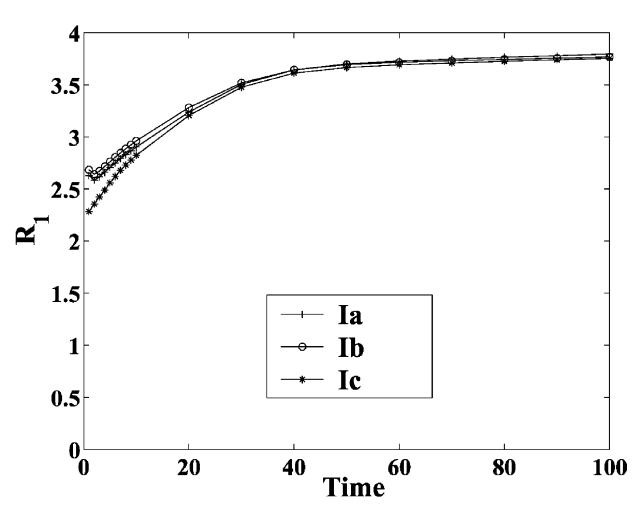
\includegraphics[width=\linewidth]{Fig5A}
\caption{Actual Figure}
\end{figure}

\begin{figure}[H]
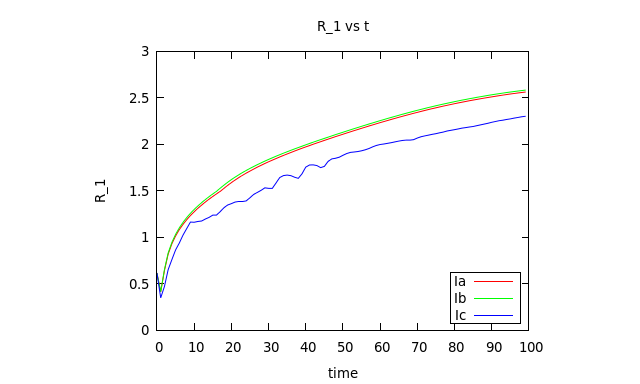
\includegraphics[width=\linewidth]{Fig5}
\caption{Reproduced Figure}
\end{figure}

\section{Number of GB bands}
A different analysis of the GB-initiated composition wave can be used for estimating the number of GB bands in the microstructure. This analysis is based on the extent of decomposition defined by:

\begin{equation}
f_D=\frac{\int_{V_b} (c_p-c_o)^2 dV}{V_b c_o (1-c_o))} 
\end{equation}

where $\mathbold{V_b}$ is the volume of interest,
By definition, $\mathbold{f_D=0}$ for a homogeneous alloy, and $\mathbold{f_D=1}$ at equilibrium.
The hypothesis we wish to test is that the GB initiated composition wave (and the associated band formation) progresses into the grain until it encounters a region that has decomposed to a significant extent. For this purpose, $\mathbold{f_D}$ is estimated separately for each of the bands in a simulation of GB-assisted SD, which is carried out with no initial composition fluctuation within the grains. 
These $\mathbold{f_D}$ values for individual bands are plotted as a function of time, and compared with similar plots for two bulk simulations (with no GB) of system Ia starting with an initial noise of $\mathbold{\delta_c = 0.04}$ and $\mathbold{\delta_c = 0.01}$.
From the figure the curve for the fourth band lies close to that for the bulk simulation with a higher initial noise $\mathbold{\delta_c = 0.04}$. This implies that a fourth band is unlikely to form in this system. Fig. \label{3A} ($1^{st}$ part) shows that this is indeed the case.
In a similar way, since fD curve for the sixth band is close to that for the bulk system with $\mathbold{\delta_c = 0.01}$, we may expect only five bands for this system. again, Fig. \label{3A} ($2^{nd}$ part) shows that this is indeed the case.

\begin{figure}[H]
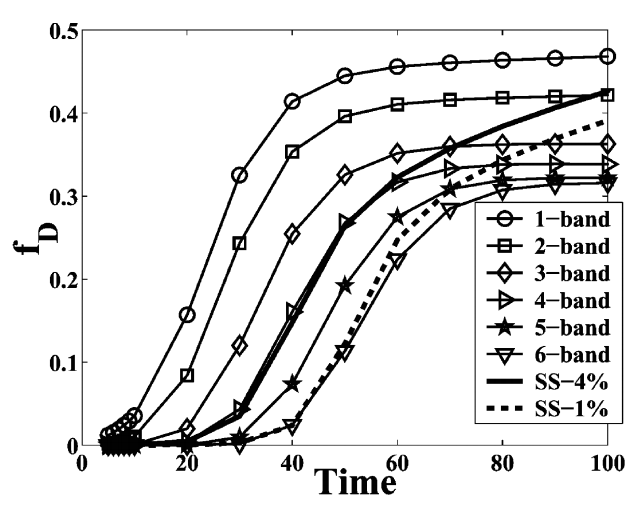
\includegraphics[width=\linewidth]{Fig6A}
\caption{Actual Figure}
\end{figure}

\begin{figure}[H]
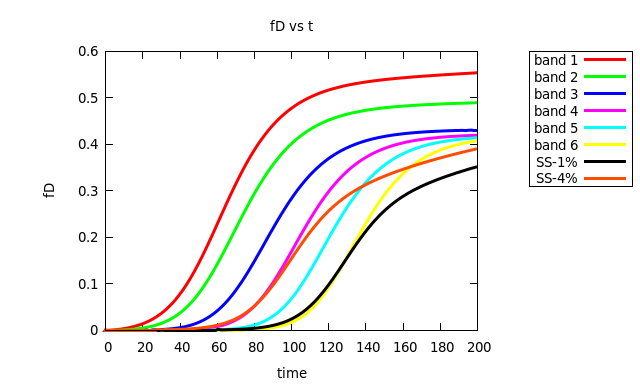
\includegraphics[width=\linewidth]{Fig6}
\caption{Reproduced Figure}
\end{figure}




\chapter{Conclusions}

\begin{enumerate}
\item We have developed a phase field model of a polycrystalline binary alloy by combining the Cahn–Hilliard model for a compositionally inhomogeneous alloy with a model of polycrystals (due to Fan and Chen).
\item We have used this model for studying GB effects on SD in systems in which the atomic mobility at GB is the same as that in the grain interior.
\item In systems in which the GB-energy of the a phase is lower than that of the $\mathbold{\beta}$ phase, the primary effect of a GB is the formation of alternating bands of the product phases parallel to the boundary. At the end of the decomposition, the microstructure exhibits these GB-bands coexisting with a normal SD microstructure in the grain interior.
\item The number of bands has been rationalized in terms of the driving force for band formation ($\mathbold{\gamma_\beta-\gamma_\alpha}$), and the strength of initial composition fluctuations. Formation of bands also effectively arrests grain growth.
\end{enumerate}

\cleardoublepage

\iffalse

% --------------------------
% Back matter
% --------------------------
{%
\setstretch{1.1}
\renewcommand{\bibfont}{\normalfont\small}
\setlength{\biblabelsep}{0pt}
\setlength{\bibitemsep}{0.5\baselineskip plus 0.5\baselineskip}
\nocite{*}
\printbibliography[nottype=online]
\printbibliography[heading=subbibliography,title={Webseiten},type=online,prefixnumbers={@}]
}
\cleardoublepage

\listoffigures
\cleardoublepage

\listoftables
\cleardoublepage

% !TEX root = ../thesis-example.tex
%
\pagestyle{empty}
\hfill
\vfill
\pdfbookmark[0]{Colophon}{Colophon}
\section*{Colophon}

This thesis was typeset with \LaTeXe.
It uses the \textit{Clean Thesis} style developed by Ricardo Langner.
The design of the \textit{Clean Thesis} style is inspired by user guide documents from Apple Inc.

Download the \textit{Clean Thesis} style at \url{http://cleanthesis.der-ric.de/}.

\cleardoublepage

\fi
% **************************************************
% End of Document CONTENT
% **************************************************
\end{document}
